\Subsection{Случайная величина}

\begin{definition}
    Случайная величина $\xi$ --- отображение  $\xi: \Omega \to \R$.
\end{definition}
\slashn
Иногда описание при помощи $\Omega, \mathbb{A}, \Pr$ даёт слишком точное, громоздкое описание. А мы хотим только суть: например сумму значений после броска двух кубиков.

Рассмотрим некую $\Omega$: $|\Omega| = m, |X| = n$, где  $X = \{x_i \mid x_i = \xi(\omega)\}$. Рассмотрим событие $A_k = \{ \omega \in \Omega \mid \xi (\omega) = x_k \}$. Тогда  $\Pr(A_k) = \sum_{\omega \in \Omega; \xi(\omega) = x_k} \Pr(\omega)$.

\begin{definition}
    $\{\Pr(A_1), \ldots, \Pr(A_n)\}$ --- распределение вероятности случайной величины $\xi$. Причем $\sum_{k=1}^n \Pr(A_k) = 1$.
\end{definition}
\slashn
А теперь пусть $B$ --- множество всех подмножеств  $X$, тогда можно перейти к пространству  $(X, B, \Pr)$. Так мы получили более простой эксперимент.
\Subsection{Биномиальное распределение}
Вспомним, что такое схема Бернулли: пусть есть монетка, которую кидаем  $n$ раз, орел выпадает с вероятностью  $p$, решка с вероятностью  $q$. Тогда $\omega = (0,1,1,0,\ldots,0)$, в общем случае $\omega = (a_1, a_2,\ldots,a_n), a_n \in \{0,1\}$. $k \coloneqq \sum_{i=1}^n a_i$  --- количество успехов в $n$ испытаниях.

Нам кажется, что такое описание $\omega$ довольно сложно, нам хочется просто знать что-то про $k$. Тогда введем  $\xi$:  $\xi(\omega) = k$. Тогда  $X = \{0,1,2,\ldots,n\}$, а $\Pr(\xi(\omega)=w) = \binom{n}{k} p^k q^{n-k}$. 

Тогда заметим, что  $\sum_{k=0}^n \binom{n}{k} p^k q^{n-k} = (p+q)^n = 1^n = 1$. Значит, у нас нормальная вероятность. Построим тогда график.
\begin{center}
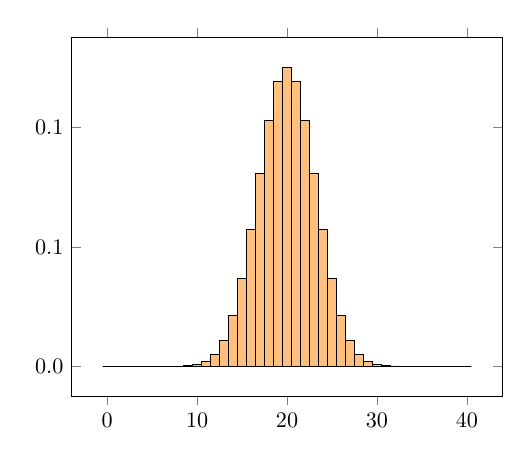
\begin{tikzpicture}[
    declare function={binom(\k,\n,\p)=\n!/(\k!*(\n-\k)!)*\p^\k*(1-\p)^(\n-\k);},
    scale=0.8
]
\begin{axis}[
    samples at={0,...,40},
    yticklabel style={
        /pgf/number format/fixed,
        /pgf/number format/fixed zerofill,
        /pgf/number format/precision=1
    },
    ybar=0pt, bar width=1
]
\addplot [fill=orange, fill opacity=0.5] {binom(x,40,0.5)}; 
\end{axis}
\end{tikzpicture}
\end{center}
\Subsection{Геометрическое распределение}
Нам интересен первый момент, когда у нас произошел фейл. Тогда пусть $\xi(\omega) = k$ --- первый момент фейла.  $\Pr(\xi(\omega)=k) = q^{k-1}\cdot p$. Тогда проверим нормировку:  $\sum_{k=1}^\infty = p\cdot q^{k-1} = p \sum_{k=1}^\infty q^{k-1} = \frac{p}{1-q} = \frac{p}{p} = 1$.
\Subsection{Гипергеометрическое распределение}
У нас есть три переменных $n, m, k$. Число предметов первого и второго сорта. $\xi(\omega)$ --- кол-во предметов 1-го сорта в выборке из  $k$ человек. $\Pr(\xi(\omega) = i) = \frac{\binom{n}{i} \binom{m}{k-i}}{\binom{n+m}{k}}$ 

У нас могут начаться проблемы из-за того, что у нас может быть задано несколько величин. Пусть $\eta$ --- произведение при броске двух кубиков.
\begin{center}
\begin{tabular}{|c|c|c|c|c|c|c|c|c|c|c|c|c|}
    \hline
     $y$ & 1 & 2 & 3 & 4 & 5 & 6 & 8 & 9 & 10 & 12 & 15 & 16 \\     \hline
     $\Pr(B)$ & $\frac{1}{36}$ & $\frac{2}{36}$ & & & & & & & & & & \\ \hline
\end{tabular}
\end{center}
\begin{definition}
Если $\forall \omega: \Pr(\xi(\omega)=x \land \eta(\omega)=y) = \Pr(\xi(\omega)=x_k) \cdot \Pr(\eta(\omega) = k)$, то случайные величины независимы.
\end{definition}
\slashn
Посмотрим на $\xi(\omega) = x_i, \eta(\omega) = y_i$. Тогда пусть  $\chi(\omega) = \eta(\omega) + \xi(\omega)$. Тогда $\Pr(\chi(\omega) = z) = \Pr(\chi(\omega) = x_i + y_i) = \sum_{k, j: x_k + y_j = z} \Pr(\xi(\omega) = x_k \land \eta(\omega) = y_k)$. Если величины независимы, то получим  под суммой $\Pr(\xi(\omega)) \cdot \Pr(\eta(\omega))$
